\chapter{线性方程组}

\section{Overview}
\begin{figure}[h]
	\centering
	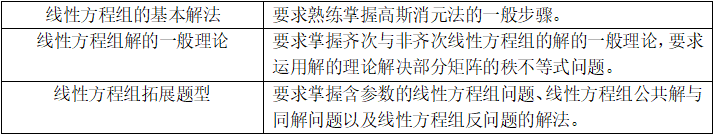
\includegraphics[scale=0.58]{8.png}
\end{figure}

\section{高斯消元法}
高斯消元法是考试中一定会考察的内容,无论是单独一个大题考察,还是嵌入在求解极大线性无关组等问题中。
注意单独考察解方程时,时间充足时建议将过程写完整,标明初等行变换的具体步骤,并且至少写出阶梯矩阵和行简化阶梯矩阵。
除此之外,需要保证计算中尽量减少错误,时间充足可以解完方程后将答案代入进行检查。

需要强调的是,不要认为本节内容很简单就放过了,实际上如果长期不计算高斯消元法很容易
造成眼高手低的窘境,因此希望各位同学熟悉高斯消元法的基本步骤并熟练应用。
\subsection{基本步骤}
一般的,对于一个由$m$个方程组成的$n$元(即变量数为$n$)线性方程组
$$\begin{cases}
	a_{11}x_1+a_{12}x_2+\cdots+a_{1n}x_n=b_1 \\
	a_{21}x_1+a_{22}x_2+\cdots+a_{2n}x_n=b_2 \\
	\cdots \\
	a_{m1}x_1+a_{m2}x_2+\cdots+a_{mn}x_n=b_m \\
\end{cases}$$
将其系数排列成矩阵
$$\begin{pmatrix}
	a_{11} & a_{12} & \cdots & a_{1n} \\
	a_{21} & a_{22} & \cdots & a_{2n} \\
	\cdots \\
	a_{m1} & a_{m2} & \cdots & a_{mn}
\end{pmatrix},$$
且记$\bm{b}=(b_1,b_2,\cdots,b_m)^\mathrm{T}$,若$\bm{b}=0$则称此方程为齐次线性方程组,否则为非齐次线性方程组。
再将$n$个未知量记为$n$元列向量$\bm{X}=(x_1,x_2,\cdots,x_n)^\mathrm{T}$,我们便可以把方程组简记为
$A\bm{X}=\bm{b}$.

令$\bm{\beta_i}=(a_{1i},a_{2i},\cdots,a_{mi})^\mathrm{T}$,即方程组系数矩阵的某一列,
则方程组还可以记为$x_1\bm{\beta_1}+x_2\bm{\beta_2}+\cdots+x_n\bm{\beta_n}=\bm{b}$,这一形式将在之后多次见到。

在以上的记号下,我们可以将解线性方程组的过程转化为矩阵的初等行变换。高斯消元法的一般步骤如下:

\centerline{线性方程组$\overset{1}{\longrightarrow}$增广矩阵$\overset{2}{\longrightarrow}$阶梯矩阵$\overset{3}{\longrightarrow}$(行)简化阶梯矩阵$\overset{4}{\longrightarrow}$解}

\begin{enumerate}
	\item 步骤1只需要将线性方程组转化为$(A, \bm{b})$的形式,得到左$n$列为系数矩阵,最后一列为列向量$\bm{b}$的$n+1$列的增广矩阵;
	\item 步骤2是通过初等行变换后,得到教材P34(1-13)的形式的矩阵——阶梯矩阵。阶梯矩阵系数全零行在最下方,并且非零行中,在下方的行的第一个非零元素一定在上方行的右侧(每行第一个非零元素称主元素);
	\item 步骤3将主元素化1后将主元素所在列的其他元素均通过初等行变换化为0即可;
	\item 步骤4中,我们分三种情况讨论:
	\begin{enumerate}
		\item 有唯一解:没有全零行,且行简化阶梯矩阵对角线上全为1,其余元素均为0,此时可以直接写出解;
		\item 无解:出现矛盾方程,即系数为0的行的行末元素不为0,此时直接写无解即可;
		\item 有无穷解:非上述情况。此时设出自由未知量将其令为$k_1,k_2,\cdots$然后代入增广矩阵对应的方程组即可。注意选取自由未知量时,选取没有主元素出现的列对应的未知量会与标准答案更贴近(如教材P33选取$x_2$、$x_5$),当然选择其他作为自由未知量也可以。
	\end{enumerate}
\end{enumerate}

\subsection{其他方法}
实际上我们还有其他方式解线性方程组,例如在系数矩阵可逆时直接求逆矩阵或者使用 Cramer 法则求解。
这些方法在之前相关章节已经讲述,此处不再展开。

\subsection{习题}
\centerline{\heiti A组}
\begin{enumerate}
	\item 求齐次线性方程组$\begin{cases}
		x_1+x_2+x_3+4x_4-3x_5=0 \\
		2x_1+x_2+3x_3+5x_4-5x_5=0 \\
		x_1-x_2+3x_3-2x_4-x_5=0 \\
		3x_1+x_2+5x_3+6x_4-7x_5=0
	\end{cases}$的通解.
	\item 求非齐次线性方程组$\begin{cases}
		x_1-x_2+2x_3-2x_4+3x_5=1 \\
		2x_1-x_2+5x_3-9x_4+8x_5=-1 \\
		3x_1-2x_2+7x_3-11x_4+11x_5=0 \\
		x_1-x_2+-x_3-x_4+3x_5=3
	\end{cases}$的通解.
	\item 求解线性方程组$\begin{cases}
		x_1+x_2+x_3=1 \\ x_1+2x_2-5x_3=2 \\ 2x_1+3x_2-4x_3=5
	\end{cases}$.
	\item 已知$V_1$是线性方程组$$\begin{cases}
		3x_1+4x_2-5x_3+7x_4=0 \\
		4x_1+11x_2-13x_3+16x_4=0
	\end{cases}$$
	的解空间,$V_2$是线性方程组$$\begin{cases}
		2x_1-3x_2+3x_3-2x_4=0 \\
		7x_1-2x_2+x_3+3x_4=0
	\end{cases}$$
	的解空间,分别求$V_1 \cap V_2$与$V_1+V_2$的基和维数.
	\item 设$A=\begin{pmatrix}
		1 & -1 & -1 \\ -1 & 1 & 1 \\ 0 & -4 & 2
	\end{pmatrix}$,$\xi_1=(-1,1,-2)^\mathrm{T}$.

	(1)求满足$A\xi_2=\xi_1$及$A^2\xi_3=\xi_1$的所有$\xi_2,\xi_3$;

	(2)证明:$\xi_1,\xi_2,\xi_3$线性无关.
\end{enumerate}

\section{线性方程组解的一般理论}
本节内容非常重要,一方面这是教材前六章的一大目标,即研究线性方程组不同解的情况
的来由;另一方面在于,这一节的内容在考试中经常出现,因此希望引起重视。

注意:本章在内容排布上与教材略有区别,但教材内容都会涉及。目的在于希望大家
不是死记硬背结论,而是能够遇到变式的定理都能理解并给出证明。如果希望先按照教材思路
回顾,实际上教材本章核心就在于定理6.1-6.3,应熟练掌握其证明并深刻理解其内涵。
\subsection{线性方程组解的一般理论}
\begin{theorem}
	(线性方程组有解的充要条件)线性方程组有解的充分必要条件是其系数矩阵与增广矩阵有相同的秩.
\end{theorem}
定理的证明非常简单,将方程组视为$x_1\bm{\beta_1}+x_2\bm{\beta_2}+\cdots+x_n\bm{\beta_n}=\bm{b}$,
则有解的条件为$\bm{b}$可以被$\bm{\beta_1},\cdots,\bm{\beta_n}$线性表示,这等价于
向量组$(\bm{\beta_1},\cdots,\bm{\beta_n})$与$(\bm{\beta_1},\cdots,\bm{\beta_n},\bm{b})$等价,故定理成立。

\begin{theorem}
	当方程组有解时(注意这个前提),以下定理成立:

	\textup{1} 如果它的系数矩阵$A$的秩等于未知量的数目$n$,则方程组有唯一解;
	
	\textup{2} 如果$A$的秩小于$n$,则方程组有无穷多个解.
\end{theorem}
这一定理有一个推论:齐次线性方程组有非零解的充要条件是:它的系数矩阵的秩小于未知量的数目(对于方阵即为行列式一章描述的,有非零解充分必要条件为其行列式为0)。
定理2对应齐次线性方程组即为教材定理6.1的推论,对于非齐次的情况,注意本定理前提是方程组有解。证明时将方程组化为简化阶梯矩阵即可。
\subsection{齐次线性方程组解的一般理论}
对于齐次线性方程组$AX=0$,我们有:
\begin{theorem}
	其解空间为$\mathbf{R}^n$的子空间。
\end{theorem}
请回顾证明子空间的一般方法。在确认其为线性空间后,我们来研究该线性空间的基本性质。首先是由此引出的关于基础解系的概念。
基础解系即为齐次线性方程组解空间的一组基,且这组基的每一个线性组合都是该方程组的解、
然后我们来研究这一空间的维数:
\begin{theorem}
	矩阵$A \in M_{m \times n}(\mathbf{F})$,若$r(A) = r$,则该齐次线性方程组解空间维数为$n - r$.
\end{theorem}
该定理即为教材定理6.1,证明使用维数公式(教材定理3.2)。本定理改写为类似于维数公式的形式即为$r(A) + \dim N(A) = n$。
其中$N(A)$表示$A\bm{X}=0$的解空间。
\begin{example}
	若$n$元齐次线性方程组$AX = 0$的解都是$BX = 0$的解,证明:$r(B) \le r(A)$.
\end{example}
\begin{theorem}
	$^*$齐次线性方程组解空间的正交补是由方程组行向量为基张成的线性空间.
\end{theorem}
该定理需要用到正交补的概念,没有学习的班级可以参考教材2.9节简单理解。实际上在矩阵的秩的讲义中已经提到了这一定理。
本定理中考虑了行向量张成的行空间,以往我们考虑列空间更多。

\subsection{非齐次线性方程组解的一般理论}
对于非齐次线性方程组
\begin{equation}
	x_1\bm{\beta_1}+x_2\bm{\beta_2}+\cdots+x_n\bm{\beta_n}=\bm{b}
\end{equation}
我们将n元齐次线性方程组
\begin{equation}
	x_1\bm{\beta_1}+x_2\bm{\beta_2}+\cdots+x_n\bm{\beta_n}=0
\end{equation}
称为其导出组,则我们有:
\begin{theorem}
	如果$n$元非齐次线性方程组有解,则它的解集$U=\{\gamma_0+\eta\ |\ \eta \in W\}$.
\end{theorem}
其中$\gamma_0$为(1)的一个解(称为特解),$W$为(2)的解空间((2)的解称为通解)。
对于通解+特解,我们可以想象一个3元非齐次线性方程$ax + by + cz = d$ 和齐次线性方程$ax + by + cz = 0$。
非齐次线性方程的解显然对应一个不过原点的平面,而齐次则过原点。
我们便可以认为是齐次线性方程解平面沿着特解对应的向量平移到非齐次线性方程的解平面,这便是这一结论的几何解释。同时我们可以得到下述结论:

1. $n$元非齐次线性方程组(1)的两个解的差是它的导出组(2)的一个解。

2. $n$元非齐次线性方程组(1)的一个解与它的导出组(2)的一个解之和仍是非齐次线性方程组(1)的一个解。

这两个性质证明比较简单,实际上根据上述几何描述形象理解也不困难。上述定理与性质对应教材定理6.3,可以参看。
\begin{example}
	设$n$阶矩阵$A$的行列式$|A|\neq 0$,记$A$的前$n-1$列形成的矩阵为$A_1$,$A$的第$n$列为$b$,
	问:线性方程组$A_1X=b$是否有解?
\end{example}

\subsection{习题}
\centerline{\heiti A组}
注意,A组习题中大部分题目都比较基础,或者直接就是教材或前面叙述的定理,所以如果有足够的自信可以只考虑思路,当然如果没有把握就请仔细写下证明。

证明以下关于线性方程组解的理论的基本定理:

第一组(齐次线性方程组解空间的一般理论)
\begin{enumerate}
	\item 设矩阵 $A \in M_{m\times n}(\mathbf{F})$,若 $r(A)=r$,则齐次线性方程组 $AX=0$ 的解空间 $N(A)$ 是 $\mathbf{F}^n$ 的一个 $n-r$ 维子空间.
	
	\item 设 $A$ 为 $m \times n$ 矩阵,则

		(1)齐次线性方程组 $AX=0$ 只有零解等价于 $r(A)=n$;
		
		(2)齐次线性方程组 $AX=0$ 有非零解(无穷解)等价于 $r(A)<n$.
	
	\item 设 $A$ 为 $n$ 阶矩阵,则

		(1)齐次线性方程组 $AX=0$ 只有零解等价于 $|A|\neq 0$;

		(2)齐次线性方程组 $AX=0$ 有非零解(无穷解)等价于 $|A|=0$.
	
	第二组(非齐次线性方程组解空间的一般理论)
	
	\item 对于非齐次线性方程组 $AX=b$,下列命题等价:
		
		(1)$AX=b$ 有解;
		
		(2)$b \in R(A)$,即 $b$ 可被 $A$ 的列向量组线性表示;
		
		(3)$r(A,b)=r(A)$,即增广矩阵的秩等于系数矩阵的秩.
	
	第三组(线性方程组解的结构的一般理论)
	
	\item 设 $X_1,\ X_2,\ \dots,\ X_s$ 为齐次线性方程组 $AX=0$ 的一组解,则 $k_1X_1+k_2X_2+\dots+k_sX_s$ 也为齐次线性方程组 $AX=0$ 的解,其中 $k_1,\ k_2,\ \dots,\ k_s$ 为任意常数.
	
	\item 设 $\eta_0$ 为非齐次线性方程组 $AX=b$ 的一个解,$X_1,\ X_2,\ \dots,\ X_s$ 为齐次线性方程组 $AX=0$ 的一组解,则 $k_1X_1+k_2X_2+\dots+k_sX_s+\eta_0$ 也为非齐次线性方程组 $AX=b$ 的解.
	
	\item 设 $\eta_1,\ \eta_2$ 为非齐次线性方程组 $AX=b$ 的两个解,则 $\eta_2-\eta_1$ 为齐次线性方程组 $AX=0$ 的解.
	
	\item 设 $X_1,\ X_2,\ \dots,\ X_s$ 为非齐次线性方程组 $AX=b$ 的一组解,则 $k_1X_1+k_2X_2+\dots+k_sX_s$ 也为非齐次线性方程组 $AX=b$ 的解的充分必要条件是 $k_1+k_2+\dots+k_s=1$.
	
	\item 设 $X_1,\ X_2,\ \dots,\ X_s$ 为非齐次线性方程组 $AX=b$ 的一组解,则 $k_1X_1+k_2X_2+\dots+k_sX_s$ 为齐次线性方程组 $AX=0$ 的解的充分必要条件是 $k_1+k_2+\dots+k_s=0$.
	
	判断以下关于线性方程组解的理论的说法是否正确并说明理由:
	
	第四组(一些经典的判断题)
	
	\item 方程组 $AX=b$ 有唯一解等价于方程组 $AX=0$ 只有零解.
	
	\item 设 $A$ 是 $m \times n$ 矩阵,$B$ 是 $n \times s$ 矩阵,若 $AB=O$,则 $B$ 的列向量为方程组 $AX=0$ 的解.
	
	\item 设 $A$ 是 $n$ 阶非零矩阵,则存在非零矩阵 $B$,使得 $AB=O$ 等价于 $r(A)<n$.
	
	\item 方程组 $AX=0$ 的解为 $BX=0$ 的解,则 $r(A)\ge r(B)$.
	
	\item 方程组 $AX=0$ 与 $BX=0$ 为同解方程组等价于 $r(A)=r(B)$.
	
	接下来为正常的练习题:

	\item 设$A$为四阶矩阵,$r(A)<4$,且$A_{21}\neq 0$,求方程组$AX=0$的通解.
	\item 设$A=(\alpha_1,\alpha_2,\alpha_3,\alpha_4)$为四阶矩阵,方程组$AX=0$的通解为$X=k(1,0,-4,0)^\mathrm{T}$,求
	$A^*X=0$的基础解系.
	\item 设$A$为$n$阶实矩阵,$W=\{\beta\in\mathbf{R}^n\ |\ \alpha^\mathrm{T}A\beta=0,\ \forall \alpha\in\mathbf{R}^n\}$,证明:
	
	(1)$\dim W+r(A)=n$;

	(2)$W$为$\mathbf{R}^n$的子空间.
	\item 已知4级方阵$A=(\alpha_1,\alpha_2,\alpha_3,\alpha_4)$的列向量$\alpha_1,\alpha_2,\alpha_4$线性无关,
	且$\alpha_1=2\alpha_2-\alpha_3$,若$\beta=\alpha_1-\alpha_2+3\alpha_4$,求方程组$AX=\beta$的通解.
	\item 设四元非齐次线性方程组的系数矩阵的秩为3,已知$\eta_1,\eta_2,\eta_3$是它的三个
	解向量,且$\eta_1=(2,3,4,5)^\mathrm{T},\eta_2+\eta_3=(1,2,3,4)^\mathrm{T}$,求该方程组的通解.
	\item 设$\beta_1,\beta_2,\beta_3$是$n$元非齐次线性方程组$AX=b$的三个线性无关的解,
	且$r(A)=n-2$,求:

	(1)导出组$AX=0$的一个基础解系;

	(2)$AX=2b$的一般解.
	\item 已知$A$是一个$s\times n$矩阵,证明:线性方程组$AX=b$对任意列向量$b_{s\times 1}$都有解的充要条件是$A$行满秩.
\end{enumerate}

\centerline{\heiti B组}
\begin{enumerate}
	\item 证明:若$X_0$是$AX=b$的一个特解,$X_1,\cdots,X_p$是$AX=0$的基础解系,
	证明:
	
	(1)$X_0,X_1,X_2,\cdots,X_p$线性无关;
	
	(2)$X_0,X_0+X_1,X_0+X_2,\cdots,X_0+X_p$线性无关;
	
	(3)$AX=b$的任一个解$X$可表示为
	$$X=k_0X_0+k_1(X_0+X_1)+k_2(X_0+X_2)\cdots+k_p(X_0+X_p),$$
	其中$k_0+k_1+k_2+\cdots+k_p=1$.
	\item 设$A$为$s \times n$矩阵,且$r(A)=r$,证明:非齐次线性方程组$AX=b$至多存在$n-r+1$个线性无关的解向量.
	\item 设$A$为$m \times n$矩阵,$r(A)=m$,$B$是$m$阶可逆矩阵,已知$A$的行空间$R(A^\mathrm{T})$是方程组$CX=0$的解空间,证明:
	$BA$的行向量也是$CX=0$的一个基础解系.
	\item 设$A$是$n$阶矩阵,且$A_{11}\neq 0$,证明:方程组$AX=b$($b$为非零向量)有无穷多解的充要条件为$A^*b=0$.
	\item 若$n$阶矩阵$A$的各行、各列元素之和都为0,证明:$A$的所有元素的代数余子式都相等.
	\item 已知 $\alpha_1,\ \alpha_2,\ \dots,\ \alpha_s$ 是齐次线性方程组 $AX=0$ 的一组基础解系,向量组

	$$
	\beta_1=t_1\alpha_1+t_2\alpha_2,\ \beta_2=t_1\alpha_2+t_2\alpha_3,\ \dots,\ \beta_{s-1}=t_1\alpha_{s-1}+t_2\alpha_s
	$$
	
	试问当实数 $t_1,\ t_2$ 满足何条件时,$AX=0$ 有基础解系包含向量 $\beta_1,\ \beta_2,\ \dots,\ \beta_{s-1}$,并写出该基础解系中的其余向量.
	\item (注:本题一般形式在教材第六章补充题1)已知线性方程组$$\begin{cases}
		a_{11}x_1+a_{12}x_2+\cdots+a_{1,2n}x_{2n}=0 \\
		a_{21}x_1+a_{22}x_2+\cdots+a_{2,2n}x_{2n}=0 \\
		\cdots \\
		a_{n1}x_1+a_{n2}x_2+\cdots+a_{n,2n}x_{2n}=0 \\
	\end{cases}$$
	的一个基础解系为$(b_{11},b_{12},\cdots,b_{1,2n})^\mathrm{T},\ (b_{21},b_{22},\cdots,b_{2,2n})^\mathrm{T},\ (b_{n1},b_{n2},\cdots,b_{n,2n})^\mathrm{T}$,
	求解线性方程组$$\begin{cases}
		b_{11}x_1+b_{12}x_2+\cdots+b_{1,2n}x_{2n}=0 \\
		b_{21}x_1+b_{22}x_2+\cdots+b_{2,2n}x_{2n}=0 \\
		\cdots \\
		b_{n1}x_1+b_{n2}x_2+\cdots+b_{n,2n}x_{2n}=0 \\
	\end{cases}.$$
	\item 设$A,B\in \mathbf{F}^{n\times n}$,且$r(A)=r$,$r(B)=s$,$r\begin{pmatrix}
		A \\ B
	\end{pmatrix}=k$.

	(1)证明:满足$AX=O$的$n$阶方阵$X$全体构成$\mathbf{F}^{n\times n}$的子空间,并求其维数;

	(2)令满足$AX=O$的$n$阶方阵$X$全体构成的子空间为$V_1$,满足$BX=O$的$n$阶方阵$X$全体构成的子空间为$V_2$,
	求$V_1+V_2$的维数.

	\item 设$A$是元素全为1的$n$阶方阵.
	
	(1)求行列式$|aE+bA|$,其中$a,b$为实常数;

	(2)已知$1<r(aE+bA)<n$,试确定$a,b$满足的条件,并求下列线性子空间的维数:
	$$W=\{x\ |\ (aE+bA)x=0,\ x\in\mathbf(R)\}.$$
	\item 已知线性方程组$$\begin{cases}
		a_{11}x_1+a_{12}x_2+\cdots+a_{1n}x_n=b_1 \\
		a_{21}x_1+a_{22}x_2+\cdots+a_{2n}x_n=b_2 \\
		\cdots \\
		a_{n1}x_1+a_{n2}x_2+\cdots+a_{nn}x_n=b_n \\
	\end{cases}$$
	的系数矩阵与
	$$\begin{pmatrix}
		a_{11} & a_{12} & \cdots & a_{1n} & b_1 \\
		a_{21} & a_{22} & \cdots & a_{2n} & b_2 \\
		\cdots \\
		a_{n1} & a_{n2} & \cdots & a_{nn} & b_n \\
		b_1 & b_2 & \cdots & b_n & 0
	\end{pmatrix},$$
	秩相等,求证:上述线性方程组有解.
	\item 设$A=(a_{ij})_{m\times n}$,$b$和$X$为$m$元列向量,$Y$为$n$元列向量,证明:
	
	(1)若$AY=b$有解,则$A^\mathrm{T}X=0$的任一组解都满足$b^\mathrm{T}X=0$;

	(2)方程组$AY=b$有解的充要条件是方程组$\begin{pmatrix}
		A^\mathrm{T} \\ b^\mathrm{T}
	\end{pmatrix}X=\begin{pmatrix}
		0 \\ 1
	\end{pmatrix}$无解(其中0是$n$元零向量).
\end{enumerate}

\centerline{\heiti C组}
\begin{enumerate}
	\item 用方程组的理论证明:一个$n$次多项式不可能有多于$n$个不同的根.
	\item 相容(即有解)的线性方程组$AX=b$在怎样的条件下,其解中第$k$个未知量$x_k$都是同一个值?
	你给的条件是否是充分必要的?
\end{enumerate}

\section{利用线性方程组解的一般理论解决矩阵秩的问题}
\subsection{概述}
我们首先来看四个最为经典的问题:
\begin{example}
	利用线性方程组解的一般理论,证明以下命题:
	
	\textup{(1)}设$A,B$分别是$m \times n$和$n \times s$矩阵,且$AB=O$,证明:$r(A)+r(B)\le n$\textup{;}

	\textup{(2)}设$A$是$m \times n$实矩阵,证明:$r(A^\mathrm{T}A)=r(A)$\textup{;}

	\textup{(3)}设$A,B$分别是$m \times n$和$n \times s$矩阵,则$r(AB)\le\min\{r(A),r(B)\}$\textup{;}

	\textup{(4)}$A^2=A \iff r(A)+r(E-A)=n$,$A^2=E \iff r(A+E)+r(A-E)=n$.
\end{example}
实际上,我们解决此类问题,很多时候等式都需要拆为小于等于和大于等于同时成立进行证明,经常利用
维数公式变形的齐次线性方程组解的一般理论,将问题转化为对像与核空间的研究,然后利用包含关系
(复杂的题目可能涉及子空间交与和的维数公式)以及已知的简单秩不等式进行证明。
可能部分题目较为困难,但至少请掌握上面例题中的情况。
\subsection{习题}
\centerline{\heiti A组}
\begin{enumerate}
	\item 设$A,B$分别是$m \times n$和$n \times s$矩阵,且$r(B)=n$,证明:若$AB=O$,则$A=O$.
\end{enumerate}
\centerline{\heiti B组}
\begin{enumerate}
	\item 判断:设 $A$ 是复数域上 $m \times n$ 阶矩阵,则矩阵秩 $r\left(A^T A\right)=r(A)$.
	\item 证明:对于$m \times n$实矩阵$A$,方程$A^\mathrm{T}AX = A^\mathrm{T}b$总是有解,且$A$为方阵时,$A^\mathrm{T}AX = 0$和$AX=0$同解.
	当$r(A)=n$时求其解,并证明$A(A^\mathrm{T}A)^{-1}A^\mathrm{T}$是幂等的对称矩阵.
	\item 设$A,B,C$为$n$阶实方阵,且$BAA^\mathrm{T}=CAA^\mathrm{T}$,证明:$BA=CA$.
	\item 设$A$为数域$\mathbf{F}$上的$n$阶方阵,又设线性空间$\mathbf{F^n}$的两个
	子空间为$W_1=\{X\in\mathbf{F}^n\ |\ AX=0\}$,$W_2=\{X\in\mathbf{F}^n\ |\ (A-E)X=0\}$.
	证明:$A^2=A \iff \mathbf{F}^n=W_1\oplus W_2$.
	\item $n$阶方阵$A$,$B$满足$AB=BA$,证明:$r(AB)+r(A+B)\le r(A)+r(B)$.
	\item 请按序证明以下结论:
	
	(1)$A,B$分别是$s \times m,m \times n$矩阵,则$ABX=0$与$BX=0$同解的充要条件是$r(AB)=r(B)$;

	(2)$A,B$分别是$s \times m,m \times n$矩阵,且$r(AB)=r(B)$,则对任意的$n \times t$矩阵都有$r(ABC)=r(BC)$;

	(3)设$A$是$n$阶方阵,则存在正整数$k$使得$r(A^k)=r(A^{k+1})=r(A^{k+2})=\cdots$,且对任意正整数$m$,有$r(A^n)=r(A^{n+m})$.
\end{enumerate}
\centerline{\heiti C组}
\begin{enumerate}
	\item 已知$A$是$n$阶对称矩阵,$\beta$为$n$元非零列向量,$B=\begin{pmatrix}
		A & \beta \\ \beta^\mathrm{T} & 0
	\end{pmatrix}$,证明:

	(1)若$r(A)=n$,则$B$可逆的充要条件是$\beta^\mathrm{T}A^{-1}\beta \neq 0$;

	(2)若$r(A)=r$,则$r(B)=r$的充要条件是方程组$\begin{cases}
		AX=\beta \\ \beta^\mathrm{T}X=0
	\end{cases}$有解;

	(3)若$r(A)=n-1$,则$B$可逆的充要条件是$AX=\beta$无解.
\end{enumerate}

\section{线性方程组拓展题型}
\subsection{含参数的线性方程组问题}
此类问题一般考察对于含参数的线性方程组,参数取值如何时有解/无解/有唯一解等。
此类问题一般有两种解法,一种是直接对系数矩阵做高斯消元法,另一种是考察系数矩阵行列式
是否为0(特别是系数矩阵行列式为n阶特殊行列式时)。当然考察系数矩阵行列式的方法不是
通用的,因为有时候参数不在系数矩阵,或者区分非齐次线性方程组无解/有无穷解的情况。
我们来看一个简单的例子:
\begin{example}
	讨论下面方程组的解的情况,并在有解的情况下求解:$$\begin{cases}
		x_1+x_2-x_3=1 \\ 2x_1+3x_2+kx_3=3 \\ x_1+kx_2+3x_3=2
	\end{cases}.$$
\end{example}
\subsection{线性方程组同解问题}
两个线性方程组同解实际上有两种情况:

1. 两线性方程组都无解;

2. 两线性方程组都有解且有相同的解集。

我们来看两线性方程组同解的充要条件:
\begin{theorem}
	$n$元齐次线性方程组($1$)$A_{m_1 \times n}X=0$与($2$)$B_{m_2 \times n}=0$同解的
	充要条件是$r\begin{pmatrix}
		A \\ B
	\end{pmatrix}=r(A)=r(B)$.
\end{theorem}
\begin{theorem}
	$n$元非齐次线性方程组($1$)$A_{m_1 \times n}X=b$与($2$)$B_{m_2 \times n}=d$同解的
	充要条件是
	
	\textup{1. }$r(A)\neq r(A,b)$且$r(B)\neq r(B,d)$
	
	或
	
	\textup{2. }$\begin{pmatrix}
		A & b \\ B & d
	\end{pmatrix}=r\begin{pmatrix}
		A \\ B
	\end{pmatrix}=r(A)=r(A,b)=r(B)=r(B,d)$.
\end{theorem}
这两个定理的证明比较简单,作为练习。这两个定理可以用于两含参方程组同解问题的解决方法,当然应用前需要简要说明
以下这个定理。
\begin{example}
	已知方程组$$\begin{cases}
		x_1+2x_2+3x_3=0 \\ 2x_1+3x_2+5x_3=0 \\ x_1+x_2+ax_3=0
	\end{cases}$$
	与$$\begin{cases}
		x_1+bx_2+cx_3=0 \\ 2x_1+b^2x_2+(c+1)x_3=0
	\end{cases}$$
	同解,求$a,b,c$的值.
\end{example}
\subsection{线性方程组公共解问题}
公共解即为两线性方程组解集的交集,我们从齐次和非齐次讨论有公共解的条件:
\begin{theorem}
	对于$n$元齐次线性方程组\textup{(1)}$A_{m_1 \times n}X=0$与\textup{(2)}$B_{m_2 \times n}=0$有

	\textup{(1)}\textup{(1)}与\textup{(2)}有非零公共解的充要条件是$r\begin{pmatrix}
			A \\ B
		\end{pmatrix}<n$\textup{;}

	\textup{(2)}设$\eta_1,\eta_2,\cdots,\eta_s(s=n-r(B))$是\textup{(2)}的基础解系,则
	\textup{(1)}与\textup{(2)}有非零公共解的充要条件是$A\eta_1,A\eta_2,\cdots,A\eta_s$线性相关\textup{;}

	\textup{(3)}设$\gamma_1,\gamma_2,\cdots,\gamma_t(s=n-r(A))$是\textup{(1)}的基础解系,
	$\eta_1,\eta_2,\cdots,\eta_s(s=n-r(B))$是\textup{(2)}的基础解系,则\textup{(1)}与\textup{(2)}有非零公共解的充要条件是
	$\gamma_1,\gamma_2,\cdots,\gamma_t,\eta_1,\eta_2,\cdots,\eta_s$线性相关.
\end{theorem}
\begin{theorem}
	对于$n$元非齐次线性方程组\textup{(1)}$A_{m_1 \times n}X=b$与\textup{(2)}$B_{m_2 \times n}X=d$,若\textup{(1)}与\textup{(2)}都有解,则

	\textup{(1)}\textup{(1)}与\textup{(2)}有公共解的充要条件是$r\begin{pmatrix}
			A \\ B
		\end{pmatrix}=\begin{pmatrix}
			A & b \\ B & d
		\end{pmatrix}$\textup{;}

	\textup{(2)}若$r(B)=s$,且$\eta_1,\eta_2,\cdots,\eta_{n-s+1}$是\textup{(2)}的$n-s+1$个线性无关的解,则
	\textup{(1)}与\textup{(2)}有公共解的充要条件是$b$是$A\eta_1,A\eta_2,\cdots,A\eta_{n-s+1}$的凸组合,即
	存在数$k_1,k_2,\cdots,k_{n-s+1}$使得
	$$b=k_1A\eta_1+k_2A\eta_2+\cdots+k_{n-s+1}A\eta_{n-s+1},$$
	其中$k_1+k_2+\cdots+k_{n-s+1}=1$\textup{;}
	
	\textup{(3)}若$r(A)=t$,$r(B)=s$,$\gamma_1,\gamma_2,\cdots,\gamma_{n-t+1}$是\textup{(1)}的$n-t+1$个线性无关的解,
	$\eta_1,\eta_2,\cdots,\eta_{n-s+1}$是\textup{(2)}的$n-s+1$个线性无关的解,则\textup{(1)}与\textup{(2)}有公共解的充要条件是
	存在数$k_1,k_2,\cdots,k_{n-t+1}$和$l_1,l_2,\cdots,l_{n-s+1}$使得
	$$k_1\gamma_1+k_2\gamma_2+\cdots+k_{n-t+1}\gamma_{n-t+1}-l_1\eta_1-l_2\eta_2-\cdots-l_{n-s+1}\eta_{n-s+1}=0,$$
	其中$k_1+k_2+\cdots+k_{n-t+1}=1$,$l_1+l_2+\cdots+l_{n-s+1}=1$.
\end{theorem}
以上两个定理的证明作为练习。当然这两个定理无需记忆,只需要通过证明理解其含义即可。下面我们看一个简单的例子:
\begin{example}
	设四元齐次线性方程组\textup{(1)}为$$\begin{cases}
		2x_1+3x_2-x_3=0 \\ x_1+2x_2+x_3-x_4=0
	\end{cases}.$$已知另一个四元齐次线性方程组\textup{(2)}的基础解系为
	$$\alpha_1=(2,-1,a+2,1)^\mathrm{T},\alpha_2=(-1,2,4,a+8)^\mathrm{T}.$$

	\textup{(1)}求方程组\textup{(1)}的一个基础解系;

	\textup{(2)}当$a$为何值时,方程组\textup{(1)}和\textup{(2)}有非零公共解,并求出非零公共解.
\end{example}
\subsection{线性方程组反问题}
此类问题即已知方程组的解,要给出原方程组。对于齐次的情形,如果大家还记得系数矩阵行向量空间与解空间的
正交补关系,此类题目是容易解决的。对于非齐次线性方程组,则先利用通解得到其导出齐次线性方程组,然后将
特解代入得到需要求的非齐次线性方程组。
\begin{example}
	已知$\alpha_1=(1,2,-1,0,4)^\mathrm{T},\alpha_2=(-1,3,2,4,1)^\mathrm{T},\alpha_3=(2,9,-1,4,13)^\mathrm{T}$,
	且有$W=L(\alpha_1,\alpha_2,\alpha_3)$.

	\textup{(1)}求以$W$为解空间的一个齐次线性方程组;

	\textup{(2)}求以$W'=\{\eta+\alpha\ |\ \alpha\in W\}$为解集的一个非齐次线性方程组,其中$\eta=(1,2,1,2,1)^\mathrm{T}$.
\end{example}
\subsection{习题}
\centerline{\heiti A组}
\begin{enumerate}
	\item 设$A \in \mathbf{F}^{m \times n},B \in \mathbf{F}^{(n-m) \times n}(m<n)$,
	$V_1,V_2$分别为齐次线性方程组$AX=0$和$BX=0$的解空间,证明:$\mathbf{F}^n=V_1\oplus V_2$的解的
	充要条件是$\begin{pmatrix}
		A \\ B
	\end{pmatrix}X$=0只有零解.

	注:本题是吴志祥老师2020-2021期中考试第一题的解题原理,但那题数据凑得不好因此是个错题,
	所以我们没有给具体的例子,而是给出原理要求证明,希望同学们碰到两方程组解空间互为补空间
	的题目会用这种方式解决.
	\item 齐次线性方程组$$\begin{cases}
		x_2+ax_3+bx_4=0 \\ -x_1+cx_3+dx_4=0 \\ ax_1+cx_2-ex_4=0 \\ bx_1+dx_2+ex_3=0
	\end{cases}$$
	的一般解以$x_3,x_4$作为自由未知量.

	(1)求$a,b,c,d,e$满足的的条件;

	(2)求齐次线性方程组的基础解系.
\end{enumerate}

\centerline{\heiti B组}
\begin{enumerate}
	\item 如果齐次线性方程组$$\begin{cases}
		x_1+x_2+bx_3-x_4+x_5=0 \\
		2x_1+3x_2+x_3+x_4-2x_5=0 \\
		x_2+ax_3+3x_4-4x_5=0 \\
		-3x_1-3x_2-3bx_3+bx_4+(a+2)x_5=0
	\end{cases}$$
	的解空间是3维的,试求$a,b$的值与解空间的基,解空间可能为2维吗?
	\item 设$W_1,W_2$分别为$n$元齐次线性方程组$AX=0$和$BX=0$的解空间,试构造两个$n$元
	齐次线性方程组,使它们的解空间分别为$W_1 \cap W_2$和$W_1+W_2$.
	\item 已知方程组$$\begin{cases}
		x_1+x_2+ax_3+x_4=1 \\ -x_1+x_2-x_3+bx_4=2 \\ 2x_1+x_2+x_3+x_4=c
	\end{cases}$$与$$\begin{cases}
		x_1+x_4=-1 \\ x_2-2x_4=d \\ x_3+x_4=e
	\end{cases}$$同解,求$a,b,c,d,e$.
	\item 设有两个非齐次线性方程组(1)和(2),它们的通解分别是$X=\gamma+t_1\eta_1+t_2\eta_2=\delta+k_1\xi_1+k_2\xi_2$.
	其中$\gamma=(5,-3,0,0)^\mathrm{T},\eta_1=(-6,5,1,0)^\mathrm{T},\eta_2=(-5,4,0,1)^\mathrm{T},
	\delta=(-11,3,0,0)^\mathrm{T},\xi_1=(8,-1,1,0)^\mathrm{T},\xi_2=(10,-2,0,1)^\mathrm{T}$,求这两个方程组的公共解.
	\item 若方程组$$\begin{cases}
		x_1+x_2+x_3=0 \\ x_1+2x_2+ax_3=0 \\ x_1+4x_2+a^2x_3=0
	\end{cases}$$与$$x_1+2x_2+x_3=a-1$$有公共解,求$a$的值及所有公共解.
\end{enumerate}

\centerline{\heiti C组}
\begin{enumerate}
	\item 讨论$b_1,b_2,\cdots,b_n(n\ge 2)$满足什么条件时,下列方程组$$\begin{cases}
		x_1+x_2=b_1 \\ x_2+x_3=b_2 \\ \cdots \\ x_{n-1}+x_n=b_{n-1} \\ x_n+x_1=b_n
	\end{cases}$$有解,并求解.
	\item 已知$A$是$s \times n$矩阵,$B$是$m \times n$矩阵,$X,a,b$分别是$n,s,m$元列向量,证明:
	
	(1)齐次线性方程组$AX=0$和$BX=0$同解的充要条件是$A$与$B$行向量等价(列向量不一定);

	(2)齐次线性方程组$AX=0$和$BX=0$解空间分别为$V_1,V_2$,证明:$V_1 \subseteq V_2$的充要条件是存在$m \times s$
	矩阵$C$使得$B=CA$;

	(3)线性方程组$AX=a$的解都是$BX=b$的解的充要条件是增广矩阵$(B,b)$的每个行向量都可以被$(A,a)$的行向量线性表示;

	(4)线性方程组$AX=a$与$BX=b$同解的充要条件是$(A,a)$与$(B,b)$行向量等价.
\end{enumerate}
